% It is an example file showing how to use the 'sigkddExp.cls' 
% LaTeX2e document class file for submissions to sigkdd explorations.
% It is an example which *does* use the .bib file (from which the .bbl file
% is produced).
% REMEMBER HOWEVER: After having produced the .bbl file,
% and prior to final submission,
% you need to 'insert'  your .bbl file into your source .tex file so as to provide
% ONE 'self-contained' source file.
%
% Questions regarding SIGS should be sent to
% Adrienne Griscti ---> griscti@acm.org
%
% Questions/suggestions regarding the guidelines, .tex and .cls files, etc. to
% Gerald Murray ---> murray@acm.org
%

\documentclass{format}
\usepackage{amssymb}
\usepackage{pifont}
\usepackage{pbox}
\usepackage{url}
\usepackage{hyperref}
\usepackage{tabularx}
\usepackage{algorithm}
\usepackage{algorithmic}

\newcommand{\cmark}{\ding{51}}
\newcommand{\xmark}{\ding{55}}

\begin{document}
%
% --- Author Metadata here ---
% -- Can be completely blank or contain 'commented' information like this...
%\conferenceinfo{WOODSTOCK}{'97 El Paso, Texas USA} % If you happen to know the conference location etc.
%\CopyrightYear{2001} % Allows a non-default  copyright year  to be 'entered' - IF NEED BE.
%\crdata{0-12345-67-8/90/01}  % Allows non-default copyright data to be 'entered' - IF NEED BE.
% --- End of author Metadata ---

\title{Harp SVM: a Parallel SVM Algorithm Based on Hadoop Using Harp}
%\subtitle{[Extended Abstract]
% You need the command \numberofauthors to handle the "boxing"
% and alignment of the authors under the title, and to add
% a section for authors number 4 through n.
%
% Up to the first three authors are aligned under the title;
% use the \alignauthor commands below to handle those names
% and affiliations. Add names, affiliations, addresses for
% additional authors as the argument to \additionalauthors;
% these will be set for you without further effort on your
% part as the last section in the body of your article BEFORE
% References or any Appendices.

\numberofauthors{2}
%
% You can go ahead and credit authors number 4+ here;
% their names will appear in a section called
% "Additional Authors" just before the Appendices
% (if there are any) or Bibliography (if there
% aren't)

% Put no more than the first THREE authors in the \author command
%%You are free to format the authors in alternate ways if you have more 
%%than three authors.

\author{
%
% The command \alignauthor (no curly braces needed) should
% precede each author name, affiliation/snail-mail address and
% e-mail address. Additionally, tag each line of
% affiliation/address with \affaddr, and tag the
%% e-mail address with \email.
\alignauthor Yiming Zou \\
       \affaddr{Indiana University Bloomington}\\
       \affaddr{107 S. Indiana Avenue}\\
       \affaddr{Bloomington, IN 47405-7000}\\
       \email{yizou@iu.edu}
\alignauthor Yueqi Tan\\
       \affaddr{Indiana University Bloomington}\\
       \affaddr{107 S. Indiana Avenue}\\
       \affaddr{Bloomington, IN 47405-7000}\\
       \email{yueqtan@umail.iu.edu}
%\alignauthor Lars Th{\o}rv\"{a}ld\titlenote{This author is the
%one who did all the really hard work.}\\
%       \affaddr{The Th{\o}rv\"{a}ld Group}\\
%       \affaddr{1 Th{\o}rv\"{a}ld Circle}\\
%       \affaddr{Hekla, Iceland}\\
%       \email{larst@affiliation.org}
}
%\additionalauthors{Additional authors: John Smith (The Th{\o}rvald Group,
%email: {\texttt{jsmith@affiliation.org}}) and Julius P.~Kumquat
%(The Kumquat Consortium, email: {\texttt{jpkumquat@consortium.net}}).}
%\date{30 July 1999}
\maketitle

\begin{abstract}
Support vector machines(SVM) are supervised learning models with associated learning algorithms that analyze data used for classification and regression analysis. Harp is good for SVM implementation but it needs to overcome synchronizing the global support vectors. In our experiment, we work on the Iterative SVM version implemented on Hadoop. In each iteration, each machine computes the support vectors and does an all-reduce to collective the whole global support vector set and treat it as the extra training data. From the result we can see that with larger number of mappers, the number of support vectors has greater gradient decent. Less iterations are needed to reach the final result which however remains the same. The speed up time of Hadoop-SVM and Harp-SVM both has an logit-linear acceleration along with the number of mappers. Harp performance is better than Hadoop since it reduces I/Os of communication.

\end{abstract}

\section{Introduction}
Machine learning is one of the most powerful areas we are interested in. It helps to solve numerous problems and are widely used in both academy and industry. There are a certain of machine learning algorithms that probably most of us are all familiar with, such as K-means, support vector machine\cite{suykens1999least}, neural networks\cite{haykin2004comprehensive} and so on. Each time we implement these algorithms, there is always the question to ask, how can we do better? Even with the same algorithm, the runtime can varies a lot depending on the method of implementation. Distributed systems\cite{tanenbaum2007distributed} pop up in late 20th century and thus give us a great way to answer the question.

Distributed system is a model whose components located on networked computers that communicate and coordinate their actions by passing messages. From the lecture in class, we have a more easy-understanding concept of it: a distributed system is a collection of independent computers that appears to its users as a single coherent system. With a distributed system, we can solve computational problem by ease, since we can allocate the jobs to multiple machines, and thus largely reduces the runtime. Distributed computing is also great for iterative problems such as PageRank\cite{page1999pagerank}. 

MapReduce\cite{dean2008mapreduce} is a programming model and an associated implementation to process and generate large data sets. We have a users specify "map" function and a "reduce" function. The map function processes a key/value pair to generate a set of intermediate key/value pairs, and the reduce function that merges all intermediate values associated with the same intermediate key. We write programs in this functional style so they are automatically parallelized and can be executed on a large cluster of commodity machines. The run-time system takes care of the details of partitioning, scheduling, handling failures, and managing communication. This greatly benefits programmer who has little experience with parallel and distributed systems to easily utilize the resources of a large distributed system.

The High Performance Computing(HPC)\cite{dowd1993high} and Grid Computing\cite{foster2003grid} are for large-scale data processing by using Application Program Interfaces(APIs) as Message Passing Interface(MPI)\cite{gropp1996high}. MapReduce helps to accelerate data access by collocating the data with the compute node. Therefore we have MapReduce implementations to control data locality. However, MapReduce only operates at the higher level. MPI gives control to the programmer and handles the mechanics of the data flow.

When dealing with large scale data set, we can choose to divide the work into many tasks, and give the task to one or more machines. When the computation is simple and uses little time to get the job done, we can only run the work on a single machine. When the computation is large and involving complex algorithm or iterations, the work is "cooperated" by the coherent system of multiple machines. Hence we have the necessarily of communication among all machines, for they need to know the current state of the on-doing job and receive commands from the master. Each single machine communicate with others by message passing.

Message passing sends a message to a process relying on the process as well as the supporting infrastructure to select and invoke the actual code to run. When we analyze the runtime of an algorithm, we also need to take into consideration of the communication cost. There are typically 2 communications of one node in a communication round: receiving messages from the neighbors in the parallel, sending new messages to its neighbors after the local computation. Let $N$ be the number of rounds, then the total times of communication of a node is $2N$. This can be very large when the number of nodes is considerable. Here we choose another way of communication called broadcast. It sends the updated message from the master node to all slaver nodes at the beginning of each round, and receive messages from all nodes at the end of a round of computation. This is much more convenient and saves I/Os.

With all the features above, there are many excellent framework for distributed applications. One of the most promising one is Apache Hadoop\cite{white2012hadoop}, which is also our focus of our course. Apache Hadoop is a software framework for distributed storage and distributed processing of very large data sets on computer clusters built from commodity hardware. The reason we love it correspond with its reliability, high efficiency and fault tolerance. Also, it is open-source and can be build on commercial machines, thus make it easy-use for both personal users and companies. It is designed for high-throughput applications, so it is very suitable for distributed computation.

Harp\cite{zhang2015harp} is a plugin to Hadoop. It provides collective communication library as well as associated data abstraction. By plugging Harp into Hadoop, we can convert MapReduce model into Map-Collective model and enable efficient in-memory communication. In this way we have parallel processes cooperate through collective communication for efficient data processing. What's more, Harp is neither a replication of MPI nor an attempt to transplant MPI into the Hadoop system.

It is highly recommended when we want to run iterative algorithms because of its high speed. For most of the algorithms, we can implement them simply on Hadoop. However, the reason we use Harp is that Harp's communication is based on memory while Hadoop is based on disk. Too many I/Os will largely reduce the performance. This results in less of runtime. Take PageRank as an example, Harp is much more faster than Hadoop on different experiment settings. We also has result from experiment on Pig showing Harp provides fast data caching and customized communication patterns among iterations\cite{wu2014integrating}. Since Hadoop and Apache open-source stacks are designed as the mainstream tools for handling big data problems, the development of a Hadoop plug-in to support Iterative MapReduce can lead to best performance.

Among of certain algorithms in machine learning, here we choose support vector machines for implementation on Harp. Support vector machines(SVM) are supervised learning models with associated learning algorithms that analyze data used for classification and regression analysis. Given a training data set, an SVM training algorithm divide the datas into several parts(mostly two) which each projects to a class it belongs. It can not only solve linear problems in machine learning but also polynomial ones. An SVM model represents every data point as a point in space, and maps them onto a plate of a new dimension. After one or several mappings, the points can finally be divided by a clear gap that is as wide as possible. For each mapping, SVM uses a mapping function. By reversing all the functions, we can go back from the single line(the dividing gap) to a curved surface that divides the original data set.\\

\textbf{Related Work}\\
When training a support vector machine, we need to find out the bound constraints and a linear equality constraint. This quadratic optimization problem may goes into many issues we need to consider in designing an SVM model\cite{joachims1999making}. When the training set is large and the learning tasks are considerable, time and memory are big limitations.  At worst time, SVMs scale badly with large data size due to the quadratic optimization algorithm and the kernel transformation\cite{meyer2015support}. SVM can also be very sensitive to the chosen parameter and noise. Making the correct choice of kernel parameters is crucial for obtaining good results, which also means that an extensive search must be conducted on the parameter space before results can be trusted, and this often complicates the task. The current implementation is only optimized for the radial basis function kernel, which might still be suboptimal for the data.

Harp is good for SVM implementation but it needs to overcome the huge amount of memory used and the computation complexity. Cascade SVM\cite{graf2004parallel} was proposed right for this challenge. Dataset is split into parts in feature space in this method. For each sub-dataset, the non-support vectors are filtered and only the support vectors are transmitted to the next round. Therefore, the margin optimization process need only the combined sub-dataset and can thus find out the support vectors. Another method proposed for parallel SVM training is that, for each subset of a dataset, it is trained with SVM and then the classifiers are combined into a final single classifier function. We also see propose in distributed SVM based on strongly connected network\cite{lu2008distributed}. In this way, a dataset is split into equal parts for each computer in a network. Then the support vectors are exchanged among the related computers. Upon the use of subSVM, there is an interesting paper develops a parallel SVM model based on MapReduce. As well as methods used before, training samples are divided into subsections, but each subsection is trained with a SVM model and libSVM\cite{chang2011libsvm} is used to train each subSVM. Then the non-support vectors will be filtered with subSVMs, and the support vectors of each subSVM are taken as the input of next layer subSVM. Finally, the global SVM model can be obtained through iterations and the output is obtained.



\section{Support Vector Machine}
\begin{figure}[htbp]
\centering
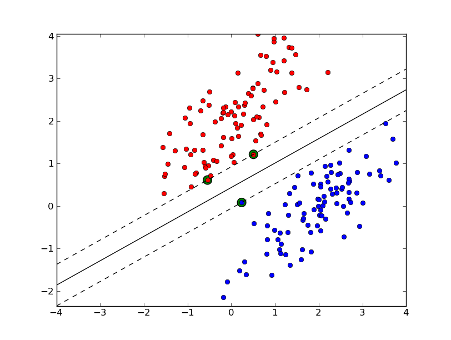
\includegraphics[width=3.0in]{image/SVM.png}
\caption{Finding the maximum gap hyperplane in SVM algorithm}
\label{SVM}
\end{figure}

Machining learning algorithms range from original K-means, Latent Dirichlet Allocation\cite{blei2003latent} to more complex ones such as Support Vector Machine, Neural Networks and Random Forest\cite{liaw2002classification}. These algorithms deal with classification or regression problems of all kinds. When choosing an algorithm to apply to a specific problem, we need to take a certain factors into consideration. Time complexity is one of the most limiting factors. When learning a large scale dataset, we often face the problem of runtime limitation. Support Vector Machine(SVM) is an important algorithm universally used is classification. It has high performance when working on certain training data and is good for simplifying polynomial problem into linear problem. In SVM algorithm, the computation time depends on large scale kernel matrix. Lots of effort have been made to optimize the runtime of SVM models.

One effective way is to reduce the number of selected features, called feature selection. Usually within a dataset there is only part of the data that we need to complete a classification. Many features are not that important in the final result and do not count for the classification. We only need to manually pick up the dependent ones regardless of the others which may take up a lot of space. This is a basic approach to reduce feature vector size\cite{weston2000feature}.
However, there may be sometime that we do not know if one feature weights over another and can not manually omit some of the features, or the feature numbers are large so selection can be lots of work. Feature subsets can then solve the problem by applying various algorithm. The most widely used algorithms are information gain\cite{kullback1951information}, 
, Gini\cite{yitzhaki1979relative}
 and correlation based feature selection\cite{hall1999correlation}.

Aside of modifying the dataset, we can also reduce time of I/O operations caused by communication. Within an iteration of SVM computation, the information of each round needs to be updated and therefore caused read and write operations. Harp is a plugin to Hadoop which specifically deal with this problem.



\section{Harp}
\begin{figure}[htbp]
\centering
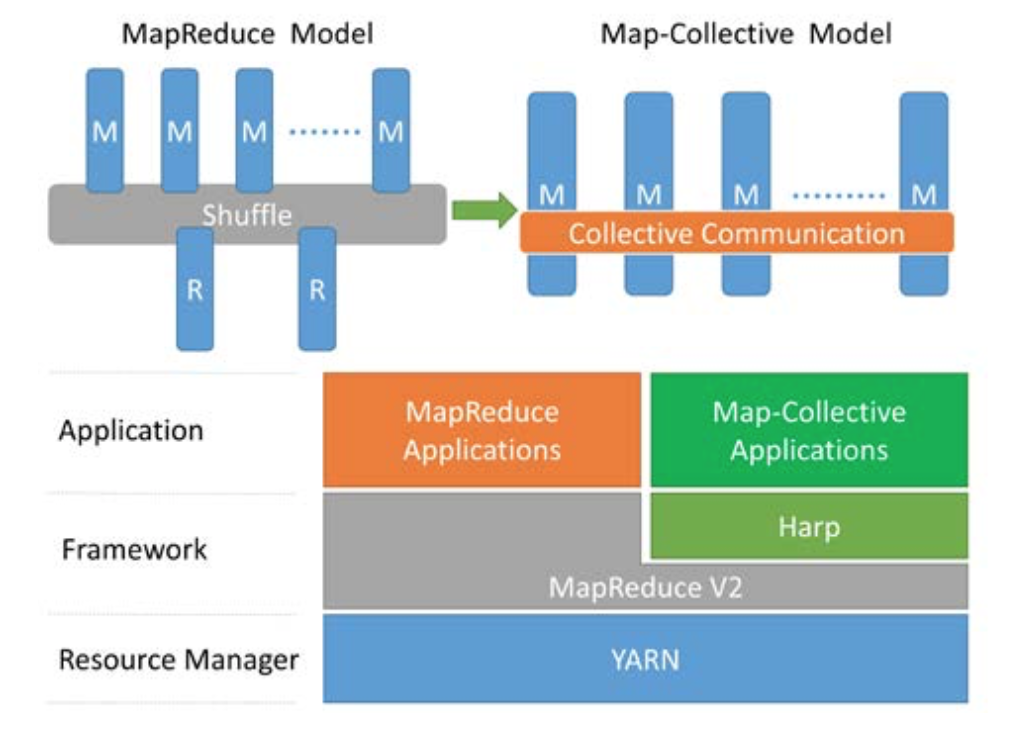
\includegraphics[width=3.0in]{image/Harp-structure.png}
\caption{Parallelism and Architecture of Harp}
\label{Harp}
\end{figure}

Harp provides collective communication library to Hadoop. It also provides associated data abstraction. Based on Hadoop, we can convert MapReduce model into Map-Collective model with the use of Harp. It is also possible to enable efficient in-memory communication, which is one of the greatest advantage Harp produces. When running iterative algorithms, runtime depends largely on communication operations arise  by information updating of each loop. Harp is therefore highly recommended because of its high speed of extracting data from cache. There is no doubt that implementing machine learning algorithms on Hadoop is an efficiency and high performance way. However, Harp works especially well on iterative models since its communication is based on memory while Hadoop is based on disk. Too many I/Os will largely increase runtime. With the implementation of Harp, we can reach high performance of algorithms and reduce runtime. Upon this, we have parallel processes cooperate through collective communication for efficient data processing. 

Benefits from Harp are plenty. When doing communication in MapReduce, the "reduce-gather-broadcast" strategy is applied through on-memory communication in frameworks such as Twister\cite{ekanayake2010twister} and Spark\cite{zaharia2010spark}. 
However, when the data set is large and so do the centroids scales, using "gather-broadcast" is no longer an efficient way. When the work loads on iterative algorithms, communication execution time is even more vital to our consideration. For each iteration, all machines need to communication with other nodes, or by simplification, with the master node. This gives out at least O(MN) operations where M is the number of machines and N is the number of iterations. By then the communication performance contributes lot to the total performance. "Collective Communication" in MPI is a good way which can abstract the communication layer out and therefore provide collective communication abstractions. 
Yet it has limitation supporting high level data abstractions and is not transparency for users. In order to improve this, we use Harp library. We can explain how Harp works as following. Harp works an optimized implementation to provide data abstractions as well as their related communication abstractions. By plugging Harp into Hadoop, we can then convert MapReduce model to Map-Collective model. This enables efficient in-memory communication between Mapper nodes whose tasks can therefore convert messages and finally work across various important data analysis applications.

\section{Iterative SVM}
\begin{figure}[htbp]
\centering
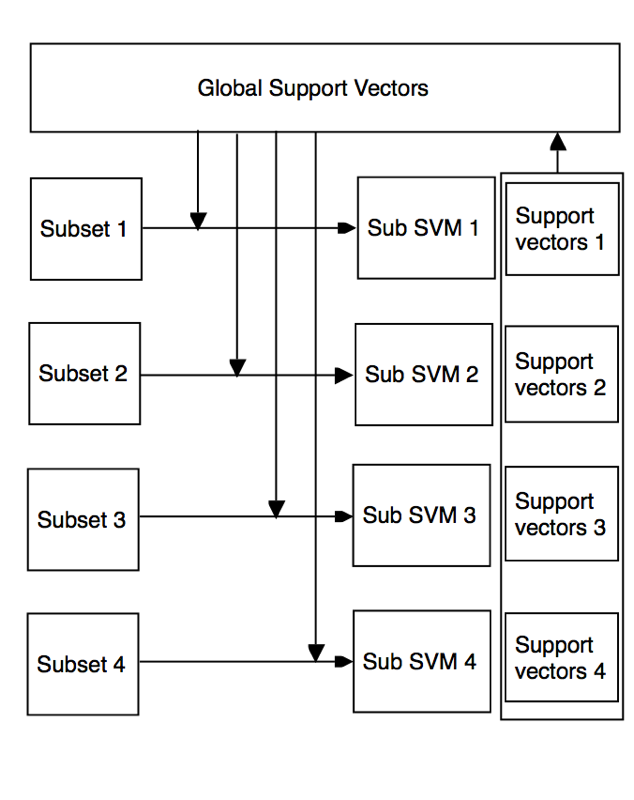
\includegraphics[width=3.0in]{image/iterativeSVM.png}
\caption{Procedure of paralleling Iterative SVM algorithm}
\label{iterativeSVM}
\end{figure}

The Iterative SVM algorithm works as Figure \ref{iterativeSVM}. The training set of the algorithm is split into subsets. Each process classifies sub dataset locally via SVM algorithm from LibSVM and gets the support vectors, and then passes the calculated support vectors to global support vectors to merge them. In Map stage of the Harp job, the subset of training set is combined with global support vectors first, and after get the new support vectors, the processes do an all-reduce to broadcast the global support vectors. And finally they can continue working on next round.

\begin{algorithm}
\caption{Iterative SVM algorithm}
\label{iterativeSVMalgorithm}
\begin{algorithmic}
\REQUIRE $dataPoints$
\ENSURE $globalSV$
\STATE split $dataPoints$ into $n$ pieces
\STATE each process gets its own piece
\STATE $globalSV=\{\}$
\FOR{$iteration=1\rightarrow n$}
\STATE combine $subDataPoints$ and $globalSV$
\STATE train data set
\STATE allreduce $SV$ to $globalSV$
\ENDFOR
\IF{Master}
\STATE output $globalSV$
\ENDIF
\end{algorithmic}  
\end{algorithm}

The pseudo code can be found in Algorithm \ref{iterativeSVMalgorithm}.

\section{Experiments}
\subsection{Data Sets}
\textbf{Fourclass}. This is a very small data sets we use for test the implementation. It has 862 data points which belong to two classes. Each data point has only two features.

\textbf{vehicle}. The vehicle data set has more data points which is 846 with 18 features. It's combined by 4 classes.

\textbf{MNIST}. This data set is a huge one with 8100000 data points in which are 784 features representing to the pixels. There are 10 classes from 0 to 9. We repeat to choose a very small part randomly from this data set and compute support vectors.

\subsection{Experimental Setup}
Experiments are done on a cluster with Intel Haswell architecture. We use 2 node each with two 12-core 24-thread Xeon E5-2670 processors. All the nodes have 128GB memory and are connected with 1Gbps Ethernet (eth) and Infiniband (ib).

\subsection{Results}
\begin{figure}[htbp]
\centering
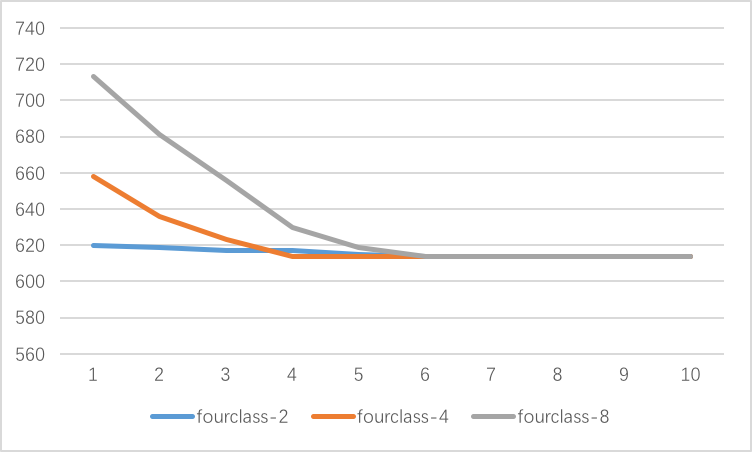
\includegraphics[width=3.0in]{image/SV-fourclass.png}
\caption{The number of support vectors versus the number of iteration on fourclass data set}
\label{SV-fourclass}
\end{figure}

\begin{figure}[htbp]
\centering
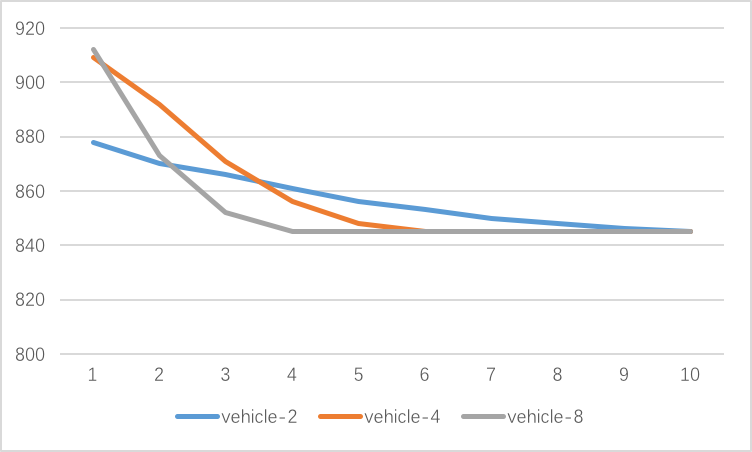
\includegraphics[width=3.0in]{image/SV-vehicle.png}
\caption{The number of support vectors versus the number of iteration on vehicle data set}
\label{SV-vehicle}
\end{figure}

\begin{figure}[htbp]
\centering
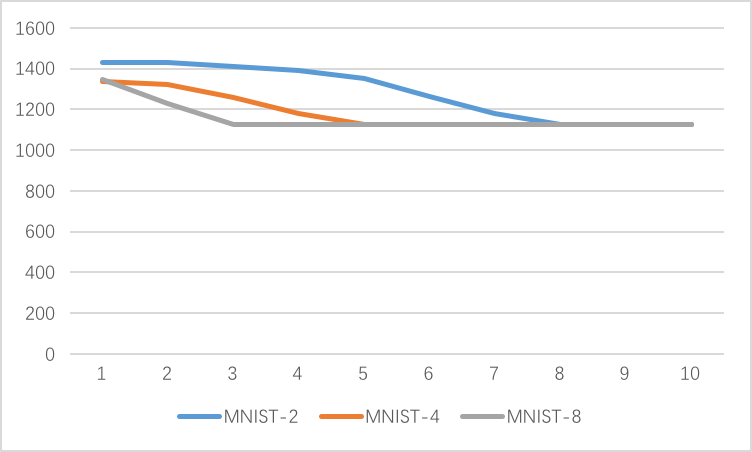
\includegraphics[width=3.0in]{image/SV-MNIST.png}
\caption{The number of support vectors versus the number of iteration on MNIST data set}
\label{SV-MNIST}
\end{figure}

From figure \ref{SV-fourclass} to figure \ref{SV-MNIST} we can see the support vectors' set becomes stable with the increase of the iteration which means that the parallel algorithm works well on training part of data and then merge the support vectors gain by the SVM algorithm. And the more mappers we use, the faster the support vectors' set becomes stable.

While, if we choose to compute by more mappers, the global support vectors at the very beginning is usually larger. That's reasonable because for small data sets, the shape of the clusters can vary from others which means that the support vectors can be very different. So after doing all-reduce, the global vector sets will be larger.

\begin{figure}[htbp]
\centering
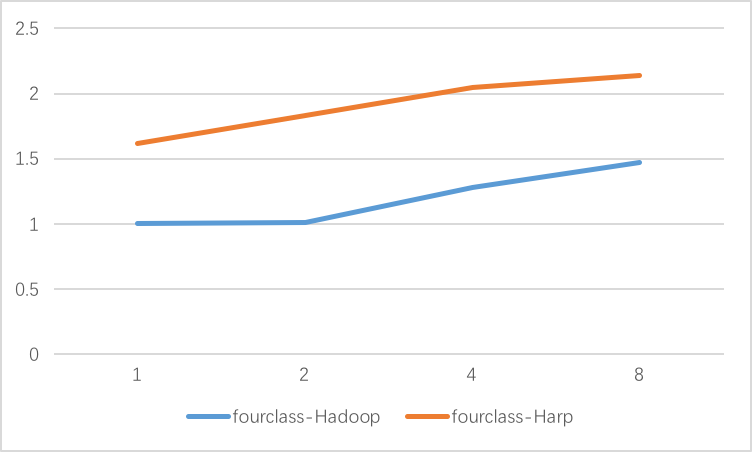
\includegraphics[width=3.0in]{image/speed-fourclass.png}
\caption{Speedup versus the number of mappers on fourclass data set}
\label{speed-fourclass}
\end{figure}

\begin{figure}[htbp]
\centering
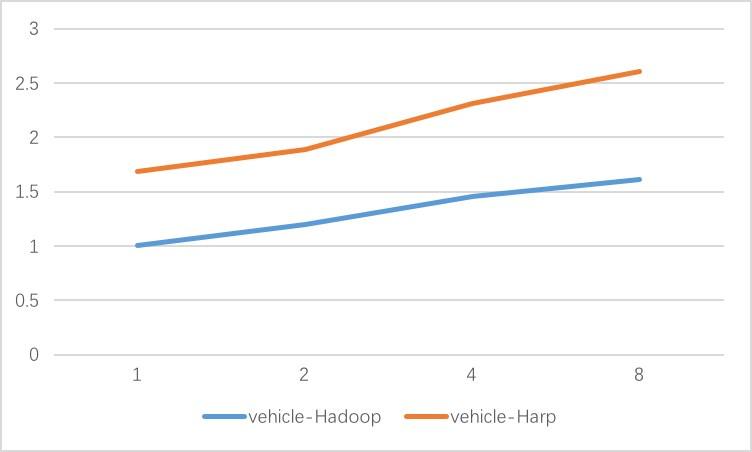
\includegraphics[width=3.0in]{image/speed-vehicle.png}
\caption{Speedup versus the number of iteration on vehicle data set}
\label{speed-vehicle}
\end{figure}

\begin{figure}[htbp]
\centering
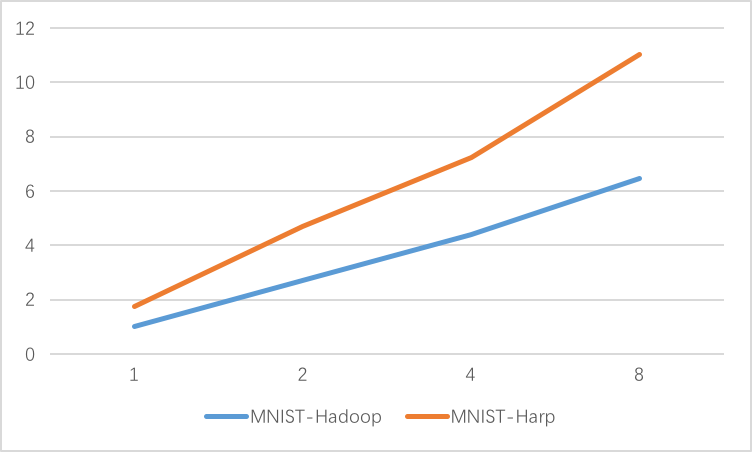
\includegraphics[width=3.0in]{image/speed-MNIST.png}
\caption{Speedup versus the number of iteration on MNIST data set}
\label{speed-MNIST}
\end{figure}

Figure \ref{speed-fourclass} to figure \ref{speed-MNIST} shows that the performance of using Harp is better than only using Hadoop. In the small data sets like fourclass and vehicle, we can see the performance improves at least 40\% and in the MNIST data set, the performance is better 80\% than the Hadoop implementation. The most saving execution time is the I/Os' time. Due to Harp can use all-reduce to synchronize data only through the cache, it will reduce much file reading and writing time which is the indispensable part in Hadoop.




\section{Conclusion}
We implement the iterative SVM algorithm based on Hadoop with the plug-in Harp. The above result has given us sufficient proof of preference using Harp to implementing SVM algorithms over other method. By using Hadoop, we fully benefit from the characteristics of distributed computing. As for multiple iterations, Harp gives us inspiration of how to communicate among the nodes with least operations. If not the best, it is a great way to balance between getting the least of necessary communication and the most of important information.

Aside of runtime, we are also concerned about the efficiency. Our result has shown the Harp implementation uses less execution time than simply Hadoop, while not sacrificing the accuracy. From the result of our implementation, we can see that support vector machine models have better performance on Hadoop by adding on the plugin Harp. The performance is optimized by 80\% of MNIST-Harp compared to MNIST-Hadoop. Hadoop generate read and write operations at each iteration while Harp stores support vectors in cache so the runtime is largely reduced. Finally, for each model we can find a global support vector set which is stable and therefore represent the output result. This is easy to understand, since Harp targets to improve the communication process in distributed computing. Moreover, we can therefore apply the presumption that Harp works better on iterative distributed computing to all related algorithms. Experiments need to be done in order to give absolute proof, though. However, for other non-iterative algorithms, we may still prefer Hadoop for its simplicity.


\section*{Acknowledgements}
Thanks to Professor Judy Qiu for giving us insightful lectures on distributed systems. Thanks to Professor Bo Peng for the deeply discussion on SVM algorithms. Thanks to all associate instructors for help on questions.

%\section{The Body of The Paper}
%Typically, the body of a paper is organized
%into a hierarchical structure, with numbered or unnumbered
%headings for sections, subsections, sub-subsections, and even
%smaller sections.  The command \texttt{{\char'134}section} that
%precedes this paragraph is part of such a
%hierarchy.\footnote{This is the second footnote.  It
%starts a series of three footnotes that add nothing
%informational, but just give an idea of how footnotes work
%and look. It is a wordy one, just so you see
%how a longish one plays out.} \LaTeX\ handles the numbering
%and placement of these headings for you, when you use
%the appropriate heading commands around the titles
%of the headings.  If you want a sub-subsection or
%smaller part to be unnumbered in your output, simply append an
%asterisk to the command name.  Examples of both
%numbered and unnumbered headings will appear throughout the
%balance of this sample document.
%
%Because the entire article is contained in
%the \textbf{document} environment, you can indicate the
%start of a new paragraph with a blank line in your
%input file; that is why this sentence forms a separate paragraph.
%
%\subsection{Type Changes and Special Characters}
%We have already seen several typeface changes in this sample.  You
%can indicate italicized words or phrases in your text with
%the command \texttt{{\char'134}textit}; emboldening with the
%command \texttt{{\char'134}textbf}
%and typewriter-style (for instance, for computer code) with
%\texttt{{\char'134}texttt}.  But remember, you do not
%have to indicate typestyle changes when such changes are
%part of the \textit{structural} elements of your
%article; for instance, the heading of this subsection will
%be in a sans serif\footnote{A third footnote, here.
%Let's make this a rather short one to
%see how it looks.} typeface, but that is handled by the
%document class file. Take care with the use
%of\footnote{A fourth, and last, footnote.}
%the curly braces in typeface changes; they mark
%the beginning and end of
%the text that is to be in the different typeface.
%
%You can use whatever symbols, accented characters, or
%non-English characters you need anywhere in your document;
%you can find a complete list of what is
%available in the \textit{\LaTeX\
%User's Guide}\cite{Lamport:LaTeX}.

%\subsection{Math Equations}
%You may want to display math equations in three distinct styles:
%inline, numbered or non-numbered display.  Each of
%the three are discussed in the next sections.

%\subsubsection{Inline (In-text) Equations}
%A formula that appears in the running text is called an
%inline or in-text formula.  It is produced by the
%\textbf{math} environment, which can be
%invoked with the usual \texttt{{\char'134}begin. . .{\char'134}end}
%construction or with the short form \texttt{\$. . .\$}. You
%can use any of the symbols and structures,
%from $\alpha$ to $\omega$, available in
%\LaTeX\cite{Lamport:LaTeX}; this section will simply show a
%few examples of in-text equations in context. Notice how
%this equation: \begin{math}\lim_{n\rightarrow \infty}x=0\end{math},
%set here in in-line math style, looks slightly different when
%set in display style.  (See next section).

%\subsubsection{Display Equations}
%A numbered display equation -- one set off by vertical space
%from the text and centered horizontally -- is produced
%by the \textbf{equation} environment. An unnumbered display
%equation is produced by the \textbf{displaymath} environment.
%
%Again, in either environment, you can use any of the symbols
%and structures available in \LaTeX; this section will just
%give a couple of examples of display equations in context.
%First, consider the equation, shown as an inline equation above:
%\begin{equation}\lim_{n\rightarrow \infty}x=0\end{equation}
%Notice how it is formatted somewhat differently in
%the \textbf{displaymath}
%environment.  Now, we'll enter an unnumbered equation:
%\begin{displaymath}\sum_{i=0}^{\infty} x + 1\end{displaymath}
%and follow it with another numbered equation:
%\begin{equation}\sum_{i=0}^{\infty}x_i=\int_{0}^{\pi+2} f\end{equation}
%just to demonstrate \LaTeX's able handling of numbering.

%\subsection{Citations}
%Citations to articles \cite{bowman:reasoning, clark:pct, braams:babel, herlihy:methodology},
%conference
%proceedings \cite{clark:pct} or books \cite{salas:calculus, Lamport:LaTeX} listed
%in the Bibliography section of your
%article will occur throughout the text of your article.
%You should use BibTeX to automatically produce this bibliography;
%you simply need to insert one of several citation commands with
%a key of the item cited in the proper location in
%the \texttt{.tex} file \cite{Lamport:LaTeX}.
%The key is a short reference you invent to uniquely
%identify each work; in this sample document, the key is
%the first author's surname and a
%word from the title.  This identifying key is included
%with each item in the \texttt{.bib} file for your article.
%
%The details of the construction of the \texttt{.bib} file
%are beyond the scope of this sample document, but more
%information can be found in the \textit{Author's Guide},
%and exhaustive details in the \textit{\LaTeX\ User's
%Guide}\cite{Lamport:LaTeX}.
%
%So far, this article has shown only the plainest form
%of the citation command, using \texttt{{\char'134}cite}.
%
%You can also use a citation as a noun in a sentence, as
% is done here, and in the \citeN{herlihy:methodology} article;
% use \texttt{{\char'134}citeN} in this case.  You can
% even say, ``As was shown in \citeyearNP{bowman:reasoning}. . .''
% or ``. . . which agrees with \citeANP{braams:babel}...'',
% where the text shows only the year or only the author
% component of the citation; use \texttt{{\char'134}citeyearNP}
% or \texttt{{\char'134}citeANP}, respectively,
% for these.  Most of the various citation commands may
% reference more than one work \cite{herlihy:methodology,bowman:reasoning}.
% A complete list of all citation commands available is
% given in the \textit{Author's Guide}.

%\subsection{Tables}
%Because tables cannot be split across pages, the best
%placement for them is typically the top of the page
%nearest their initial cite.  To
%ensure this proper ``floating'' placement of tables, use the
%environment \textbf{table} to enclose the table's contents and
%the table caption.  The contents of the table itself must go
%in the \textbf{tabular} environment, to
%be aligned properly in rows and columns, with the desired
%horizontal and vertical rules.  Again, detailed instructions
%on \textbf{tabular} material
%is found in the \textit{\LaTeX\ User's Guide}.
%
%Immediately following this sentence is the point at which
%Table 1 is included in the input file; compare the
%placement of the table here with the table in the printed
%dvi output of this document.
%
%\begin{table}
%\centering
%\caption{Frequency of Special Characters}
%\begin{tabular}{|c|c|l|} \hline
%Non-English or Math&Frequency&Comments\\ \hline
%\O & 1 in 1,000& For Swedish names\\ \hline
%$\pi$ & 1 in 5& Common in math\\ \hline
%\$ & 4 in 5 & Used in business\\ \hline
%$\Psi^2_1$ & 1 in 40,000& Unexplained usage\\
%\hline\end{tabular}
%\end{table}
%
%To set a wider table, which takes up the whole width of
%the page's live area, use the environment
%\textbf{table*} to enclose the table's contents and
%the table caption.  As with a single-column table, this wide
%table will "float" to a location deemed more desirable.
%Immediately following this sentence is the point at which
%Table 2 is included in the input file; again, it is
%instructive to compare the placement of the
%table here with the table in the printed dvi
%output of this document.
%
%
%\begin{table*}
%\centering
%\caption{Some Typical Commands}
%\begin{tabular}{|c|c|l|} \hline
%Command&A Number&Comments\\ \hline
%\texttt{{\char'134}alignauthor} & 100& Author alignment\\ \hline
%\texttt{{\char'134}numberofauthors}& 200& Author enumeration\\ \hline
%\texttt{{\char'134}table}& 300 & For tables\\ \hline
%\texttt{{\char'134}table*}& 400& For wider tables\\ \hline\end{tabular}
%\end{table*}
% end the environment with {table*}, NOTE not {table}!

%\subsection{Theorem-like Constructs}
%Other common constructs that may occur in your article are
%the forms for logical constructs like theorems, axioms,
%corollaries and proofs.  There are
%two forms, one produced by the
%command \texttt{{\char'134}newtheorem} and the
%other by the command \texttt{{\char'134}newdef}; perhaps
%the clearest and easiest way to distinguish them is
%to compare the two in the output of this sample document:
%
%This uses the \textbf{theorem} environment, created by
%the \texttt{{\char'134}newtheorem} command:
%\newtheorem{theorem}{Theorem}
%\begin{theorem}
%Let $f$ be continuous on $[a,b]$.  If $G$ is
%an antiderivative for $f$ on $[a,b]$, then
%\begin{displaymath}\int^b_af(t)dt = G(b) - G(a).\end{displaymath}
%\end{theorem}
%
%The other uses the \textbf{definition} environment, created
%by the \texttt{{\char'134}newdef} command:
%\newdef{definition}{Definition}
%\begin{definition}
%If $z$ is irrational, then by $e^z$ we mean the
%unique number which has
%logarithm $z$: \begin{displaymath}{\log_e^z = z}\end{displaymath}
%\end{definition}
%
%Two lists of constructs that use one of these
%forms is given in the
%\textit{Author's  Guidelines}.
% 
%There is one other similar construct environment, which is
%already set up
%for you; i.e. you must \textit{not} use
%a \texttt{{\char'134}newdef} command to
%create it: the \textbf{proof} environment.  Here
%is a example of its use:
%\begin{proof}
%Suppose on the contrary there exists a real number $L$ such that
%\begin{displaymath}
%\lim_{x\rightarrow\infty} \frac{f(x)}{g(x)} = L.
%\end{displaymath}
%Then
%\begin{displaymath}
%l=\lim_{x\rightarrow c} f(x)
%= \lim_{x\rightarrow c}
%\left[ g{x} \cdot \frac{f(x)}{g(x)} \right ]
%= \lim_{x\rightarrow c} g(x) \cdot \lim_{x\rightarrow c}
%\frac{f(x)}{g(x)} = 0\cdot L = 0,
%\end{displaymath}
%which contradicts our assumption that $l\neq 0$.
%\end{proof}
%
%Complete rules about using these environments and using the
%two different creation commands are in the
%\textit{Author's Guide}; please consult it for more
%detailed instructions.  If you need to use another construct,
%not listed therein, which you want to have the same
%formatting as the Theorem
%or the Definition\cite{salas:calculus} shown above,
%use the \texttt{{\char'134}newtheorem} or the
%\texttt{{\char'134}newdef} command,
%respectively, to create it.
%
%\subsection*{A Caveat for the \TeX\ Expert}
%Because you have just been given permission to
%use the \texttt{{\char'134}newdef} command to create a
%new form, you might think you can
%use \TeX's \texttt{{\char'134}def} to create a
%new command: \textit{Please refrain from doing this!}
%Remember that your \LaTeX\ source code is primarily intended
%to create camera-ready copy, but may be converted
%to other forms -- e.g. HTML. If you inadvertently omit
%some or all of the \texttt{{\char'134}def}s recompilation will
%be, to say the least, problematic.
%
%\section{Conclusions}
%This paragraph will end the body of this sample document.
%Remember that you might still have Acknowledgements or
%Appendices; brief samples of these
%follow.  There is still the Bibliography to deal with; and
%we will make a disclaimer about that here: with the exception
%of the reference to the \LaTeX\ book, the citations in
%this paper are to articles which have nothing to
%do with the present subject and are used as
%examples only.
%\end{document}  % This is where a 'short' article might terminate

%ACKNOWLEDGEMENTS are optional
%\section{Acknowledgements}
%This section is optional; it is a location for you
%to acknowledge grants, funding, editing assistance and
%what have you.  In the present case, for example, the
%authors would like to thank Gerald Murray of ACM for
%his help in codifying this \textit{Author's Guide}
%and the \textbf{.cls} and \textbf{.tex} files that it describes.

%
% The following two commands are all you need in the
% initial runs of your .tex file to
% produce the bibliography for the citations in your paper.
\bibliographystyle{abbrv}
\bibliography{references}  % sigproc.bib is the name of the Bibliography in this case
% You must have a proper ".bib" file
%  and remember to run:
% latex bibtex latex latex
% to resolve all references
%
% ACM needs 'a single self-contained file'!
%
%APPENDICES are optional
% SIGKDD: balancing columns messes up the footers: Sunita Sarawagi, Jan 2000.
% \balancecolumns
%\appendix
%Appendix A
%\section{Headings in Appendices}
%The rules about hierarchical headings discussed above for
%the body of the article are different in the appendices.
%In the \textbf{appendix} environment, the command
%\textbf{section} is used to
%indicate the start of each Appendix, with alphabetic order
%designation (i.e. the first is A, the second B, etc.) and
%a title (if you include one).  So, if you need
%hierarchical structure
%\textit{within} an Appendix, start with \textbf{subsection} as the
%highest level. Here is an outline of the body of this
%document in Appendix-appropriate form:
%\subsection{Introduction}
%\subsection{The Body of the Paper}
%\subsubsection{Type Changes and Special Characters}
%\subsubsection{Math Equations}
%\paragraph{Inline (In-text) Equations}
%\paragraph{Display Equations}
%\subsubsection{Citations}
%\subsubsection{Tables}
%\subsubsection{Figures}
%\subsubsection{Theorem-like Constructs}
%\subsubsection*{A Caveat for the \TeX\ Expert}
%\subsection{Conclusions}
%\subsection{Acknowledgements}
%\subsection{Additional Authors}
%This section is inserted by \LaTeX; you do not insert it.
%You just add the names and information in the
%\texttt{{\char'134}additionalauthors} command at the start
%of the document.
%\subsection{References}
%Generated by bibtex from your ~.bib file.  Run latex,
%then bibtex, then latex twice (to resolve references)
%to create the ~.bbl file.  Insert that ~.bbl file into
%the .tex source file and comment out
%the command \texttt{{\char'134}thebibliography}.
% This next section command marks the start of
% Appendix B, and does not continue the present hierarchy
%\section{More Help for the Hardy}
%The acmproc-sp document class file itself is chock-full of succinct
%and helpful comments.  If you consider yourself a moderately
%experienced to expert user of \LaTeX, you may find reading
%it useful but please remember not to change it.

% That's all folks!
\end{document}
